\documentclass{report}
\usepackage[margin=1in, paperwidth=8.5in, paperheight=11in]{geometry}
%Math packages%
\usepackage{amsmath}
\usepackage{amsthm}
%Spacing%
\usepackage{setspace}
\onehalfspacing
%Lecture number%
\newcommand{\lectureNum}{11}
%Variables - Date and Course%
\newcommand{\curDate}{February 7, 2017}
\newcommand{\course}{CS 241}
\newcommand{\instructor}{Kevin Lanctot}
%Defining the example tag%
%\theoremstyle{definition}%
\newtheorem{ex}{Example}[section]
%Setting counter given the lecture number%
\setcounter{chapter}{\lectureNum{}}
%Package to insert code%
\usepackage{listings}
\usepackage{courier}
\usepackage{xcolor}
\lstset { %
    tabsize=2,
    breaklines=true,
    language=C++,
    backgroundcolor=\color{blue!8}, % set backgroundcolor
    basicstyle=\footnotesize\ttfamily,% basic font setting
}
%Package for images%
\usepackage{graphicx}

\begin{document}
%Note title%
\begin{center}
\begin{Large}
\textsc{\course{} | Lecture \lectureNum{}}
\end{Large}
\end{center} 
\noindent \textit{Bartosz Antczak} \hfill
\textit{Instructor: \instructor{}} \hfill
\textit{\curDate{}}
\rule{\textwidth}{0.4pt}
% Actual Notes%
\section{Non-deterministic Finite Automata (NFA)}
The key difference found in NFA's is that \textit{two or more edges leaving the same state can have the same label and lead to different states}. This means that the next state is non-deterministic (i.e., there exists a state of possible states rather than a single state).
\begin{figure}[ht]
\begin{center}
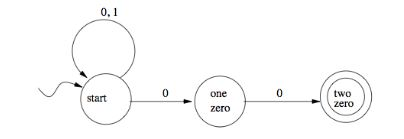
\includegraphics[scale=1]{nfa.jpg}
\end{center}
\caption{An example of an NFA. From Prof. Lanctot's slides.}
\end{figure}
Consider the input 010, running it through the NFA $\ell$, we get:
\begin{itemize}
\item $\varepsilon$ $S$
\item 0 $\{S, 10\}$
\item 1 $\{S\}$
\item 0 $\{S, 10\} \cap \{20\} = \emptyset$
\end{itemize}
Ergo $101 \not\in \ell$.\\
When working with NFA's, we don't ask ``what state are we in?". Instead, we ask
\begin{center}
\textit{What set of states are we in?}
\end{center}
One can consider a human as an NFA. We experience different states at the same time, for instance, we can be happy about finishing an assignment but sad at the same time because we missed another assignment.\\
\subsection{Comparisons with a DFA}
\begin{itemize}
\item A language is accepted in an NFA and DFA if at least one path leads to an accepting state
\item DFA's are easier to implement
\item NFA's are simpler because they tend to have less states than a corresponding DFA; however, NFA's are slower because they require set data types, which take longer to process
\end{itemize} \newpage
\subsection{Transducers}
It's an \textit{extension}. It allows to provide an output on any transition:
\begin{figure}[ht]
\begin{center}
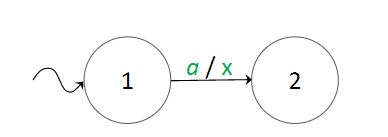
\includegraphics[scale=0.6]{transducer.jpg}
\end{center}
\caption{On transition $a$, output $x$. Courtesy of Prof. Lanctot's slides.}
\end{figure}
\subsection{Epsilon-Non-Deterministic-Finite-Automata}
An $\varepsilon-$NFA allows the use of $\varepsilon-$transitions (i.e., a transition that occurs without consuming any input:
\begin{figure}[ht]
\begin{center}
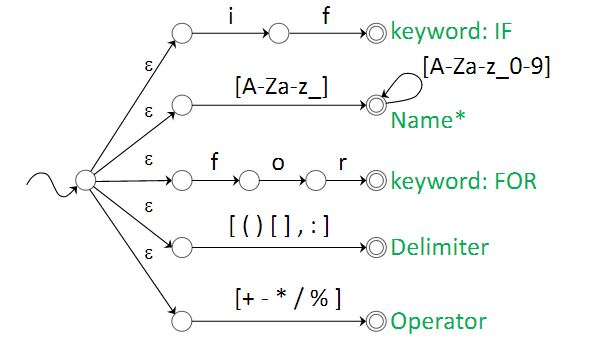
\includegraphics[scale=0.6]{enfa.jpg}
\end{center}
\caption{An $\varepsilon-$NFA. Courtesy of Prof. Lanctot's slides.}
\end{figure}

%END%
\end{document}